\chapter{Heliocentric Transfer Results}

% **************************** Define Graphics Path **************************
\ifpdf
    \graphicspath{{Chapter4/Figs/Raster/}{Chapter4/Figs/PDF/}{Chapter4/Figs/}}
\else
    \graphicspath{{Chapter4/Figs/Vector/}{Chapter4/Figs/}}
\fi

In this chapter the two dimensional and three dimensional time and fuel optimal problems are solved in the heliocentric coordinate system. Both nuclear and solar electric propulsion system models have been considered. The results are presented and analyzed. 
\section{Electrical power models}
These power models are required to determine the maximum thrust available from the electric propulsion system as follows,
\begin{align}
	T_{max}=\frac{2P\eta}{g_0 I_{sp}}
\end{align}
\subsection{Nuclear electric propulsion}
This type of propulsion system is powered by a nuclear reactor. The power output is roughly constant. For a conventional electric thruster, the thrust produced and specific impulse can be assumed to be constant. 
\subsection{Solar electric propulsion}
This form of power system is typically powered by solar arrays that generate electric power. It is assumed that the panels are controlled to face the sun at all times except during eclipses when zero power is available.
\subsubsection{Inverse square model}
This is the simplest model and is usually taken as the first approximation for the thrust produced. The power produced varies as the inverse square of the distance from the sun. It is assumed that the thrust varies linearly with the power supply and that the specific impulse is constant.
\subsubsection{Coverstone-Carroll model}
This is a significantly more complex model and accounts for the saturation of power generation as the solar distance decreases. This is obtained from a fit based on experimental data. More details on the model are available in the paper by \cite{williams_benefits_1997}. The model is as follows,
\begin{align}
	a_1&=0.7119713\\
	a_2&=0.4089753\\
	a_3&=-0.0783905\\
	a_4&=-0.0201896\\
	a_5&=0.0623406\\
	P&=\frac{P_0}{r^2}\bigg[\frac{a_1+\frac{a_2}{r}+\frac{a_3}{r^2}}{1+a_4 r+a_5 r^2}\bigg]\\
	\text{Where, }P_0&=1366W/m^2
\end{align}
\subsubsection{Alternative models}
From the mathematical formulation provided in the previous chapter, since the maximum allowable thrust and specific impulse are external parameters to the system of equations, it is possible to define any custom piecewise smooth variation for the aforementioned quantities. These can be integrated into the dynamics of the problem and the corresponding optimal trajectories can be obtained.
\section{Two dimensional time-optimal results}
This section presents the results of time-optimal transfers between two heliocentric orbits. 
\subsection{Model validation}
The code and mathematical formulation are validated by solving a well documented problem of a 1AU to 1.5AU transfer for a 1000kg NEP spacecraft with 1N thrust and $I_{sp}$ of 6000s. 
\begin{figure}[H]
	\centering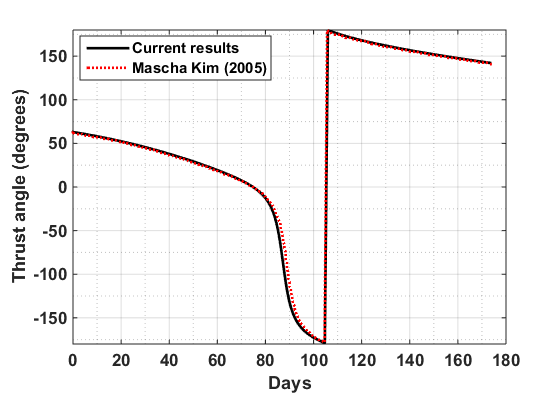
\includegraphics[width=0.625\linewidth]{Results_Compare_bold.png}
	\caption{Thrust angle profile compared with \cite{kim_continuous_2005}.}
	\label{validate_fig}
\end{figure}
The corresponding time-optimal trajectory is as follows,
\begin{figure}[H]
	\centering\includegraphics[width=0.625\linewidth]{Traj_EtoM.png}
	\caption{1AU to 1.5AU minimum time transfer.}
	\label{validate_traj}
\end{figure}
This is a classic problem that has been solved by both direct \citep{arthur._e_applied_1975} and indirect \citep{kim_continuous_2005} methods. As seen from figure \ref{validate_fig}, it is seen that the current solution strategy and mathematical formulation closely match the values from literature. This provides confidence for the proposed strategy which makes use of differential evolution.
The blue arrows depict the instantaneous thrust vector. This plot reveals that there is a large rotation of the thrust vector required during the mid portion of the trajectory. Due to the requirement of time-optimality, there is a substantial thrust component off the tangent with the thruster operating for a longer duration. This leads to higher fuel consumption but the flight duration is minimized. These trajectories may be suitable for human missions in outer space.
\subsection{Parametric studies - Circle to circle transfers}
The following is the result of a circle to circle transfers from 1AU to 1.5AU with varying thrust levels and specific impulse values. The following results are obtained.
\begin{figure}[H]
	\centering\includegraphics[width=1.00\linewidth]{Transtime_Isp.eps}
	\caption{Transfer time with varying $I_{sp}$.}
	\label{transtime_isp}
\end{figure}
From figure \ref{transtime_isp}, it is visible that the transfer time varies by about 50 days when the specific impulse is varied from 1500 to 6000. This indicates that the flight duration variation for higher specific impulse is relatively less sensitive. For varying acceleration levels, it is clear that the transfer time is highly sensitive. A factor of 8 reduction in acceleration led to an increase in flight duration by a factor of 4.\\
For very low thrust levels, the transfer takes the form of multiple revolutions around  the sun. These types of orbits are challenging to solve using the direct approach in the Cartesian coordinate system. The approach followed in this investigation faces no such issues to the solution.
\begin{figure}[H]
	\centering\includegraphics[width=1.00\linewidth]{fuelfrac_Isp.eps}
	\caption{Fuel fraction with varying $I_{sp}$.}
	\label{fuelfrac_isp}
\end{figure}
Figure \ref{fuelfrac_isp} shows the dependence of the propellant fraction on the specific impulse in the minimum time formulation. As expected, lower specific impulse leads to a high propellant consumption. The most important observation is that the propellant consumption stagnates and reaches a minimum limiting value for very low acceleration levels. This suggests that lowering the thrust hoping to achieve lower fuel fractions at the cost of flight duration is a strategy that provides diminishing returns beyond a certain extent. 
\section{Two dimensional fuel-optimal transfers}
These type of transfers allow for the spacecraft to coast with the thrusters switched off. At the expense of a higher flight duration, significant savings in terms of propellant can be achieved. The flight duration of the corresponding minimum time problem is the lower limit of the flight duration for this case. If  the two flight durations are equal, then the fuel-optimal and time-optimal solutions coincide. If the flight duration for the fuel-optimal case is set to a value lower than the minimum time, no solution can be found. Setting a flight duration greater than the minimum time value leads to solutions with coasting. The objective of this work is to ensure that the coast arises naturally from the solution procedure with no information supplied by the user. This is to avoid the requirement of the knowledge of the structure of the control as there can be trajectories with multiple coast phases.\\
\subsection{A typical Earth-Mars fuel-optimal trajectory}
The trajectory for a 400 day fuel-optimal Earth-Mars orbit transfer with a 2000s $I_{sp}$ and a thrust level of 236mN has been generated to demonstrate coasting.
\begin{figure}[H]
	\centering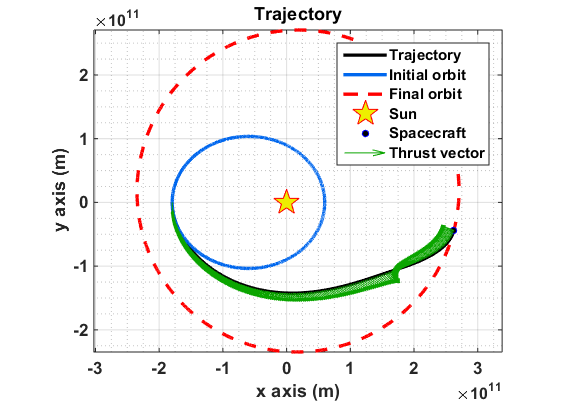
\includegraphics[width=1.00\linewidth]{Sample_Traj.eps}
	\caption{Fuel fraction with varying $I_{sp}$.}
	\label{sampletraj_fuelopt}
\end{figure}
\nomenclature[z-AU]{AU}{Astronomical Unit - $149.6\times 10^11$m}
Several important features can be observed in figure \ref{sampletraj_fuelopt}. During the start of the orbit, the thrust is radially inward and has a small retrograde component which gradually rotates to a tangential value. This maneuver occurs to enable longer thrusting in a higher velocity region closer to the sun. If the flight duration is increased, this tendency disappears. The initial thrust phase is followed by a coast duration. Here, the spacecraft flies in a Keplerian orbit. No information is provided to the numerical method a-priori about the arc location and duration of the coast. It is automatically determined. The final leg of the trajectory is a thrusting phase with a radially inward thrust. This is to circularize the final orbit around the sun at 1.524AU. The rotation of the thrust vector is seen to be very gradual. This implies that very low thrust, precision attitude control thrusters can be made use of. The attitude control requirement is estimated to be in the range of micro-Newtons to a few milli-Newtons depending on the size and shape of the spacecraft. This can be performed by smaller auxiliary electric thrusters.
\subsection{Power model comparison for outward transfer}
Here, a 200 day fuel-optimal transfer from 1AU to 1.524AU for a 1000kg spacecraft with a 1N, 2000s $I_{sp}$ thruster is used to demonstrate the differences between the various power models.
\begin{figure}[H]
	\centering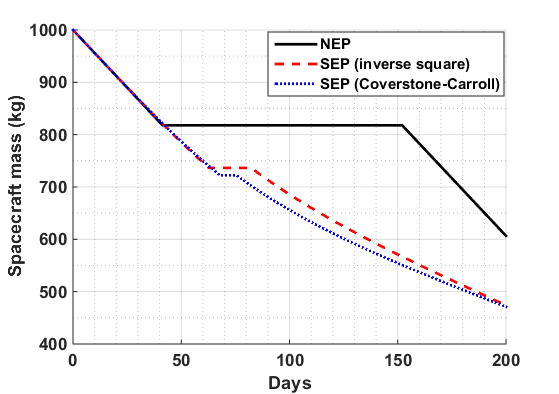
\includegraphics[width=1.00\linewidth]{Spacecraft_mass.eps}
	\caption{Spacecraft mass profile - fuel-optimal transfer.}
	\label{sc_massvar}
\end{figure}
Figure \ref{sc_massvar} shows the spacecraft instantaneous mass profile under different power models. It is seen that NEP has an advantage of over $10\%$ in comparison to both SEP models used. The coast duration is also seen to be much larger. The inverse square dependency on thrust is visible for the SEP models as the slope of the mass profile in the final thrust phase is seen to vary in a decreasing fashion as the spacecraft moves away from the sun.
\begin{figure}[H]
	\centering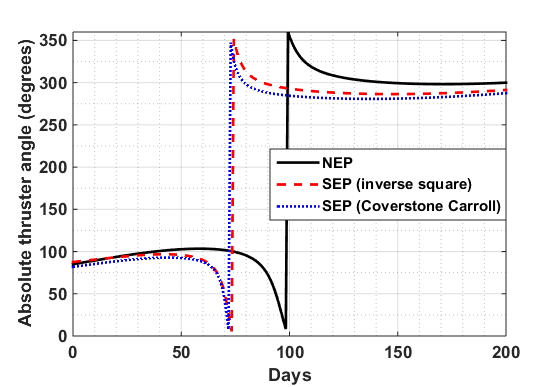
\includegraphics[width=1.00\linewidth]{Thruster_angle.eps}
	\caption{Thrust angle profile - fuel-optimal transfer.}
	\label{sc_controlang}
\end{figure}
Figure \ref{sc_controlang} shows the variation of the absolute thrust angle. It is clearly visible that the rapid change in thrust direction occurs in the middle of the coast duration. Since the thruster is inactive in this phase, there are no attitude control requirements and only the initial and final phases of the trajectory count for attitude control requirement determination. This implies that the fuel-optimal trajectory is much more benign than the time-optimal trajectory in terms of maximum attitude control requirements. micro-Newton thrust levels are sufficient to achieve this profile depending on the spacecraft mass and moment of inertia. Accurate determination of the attitude control requirements and dynamics will require a detailed 6DOF simulation.
\begin{figure}[H]
	\centering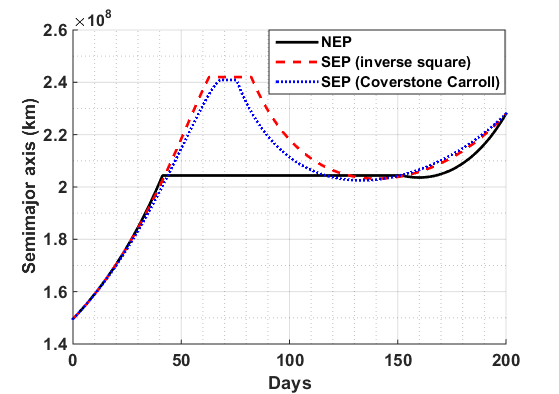
\includegraphics[width=1.00\linewidth]{Semimaj_axis.eps}
	\caption{Semi-major axis variation - fuel-optimal transfer.}
	\label{sc_semimaj}
\end{figure}
Figure \ref{sc_semimaj} shows the semi-major axis variation with time for the same transfer with different power models. It is seen that both the solar electric models drive the semi-major axis to a high level and then thrust to reduce it to the required level. This is due to the 200 day flight duration that has been specified. The NEP spacecraft on the other hand has a much longer coast and the increase in semi-major axis is much lesser. Semi-major axis is representative of the energy state of the spacecraft. It is evident that for this outward transfer, NEP does not waste much energy in comparison to SEP models. From the figure, even the NEP model shows a slight dip in semi-major axis after the end of the coast. This suggests that a modest increase in flight time will eliminate this loss. For the case of SEP, much longer flight durations are needed for the propellant consumption to approach NEP levels.
\subsection{Parametric study results}
For the same problem as before, the flight duration is varied from 200 days to 300 days and the corresponding fuel-optimal results are presented as a parametric study.
\begin{figure}[H]
	\centering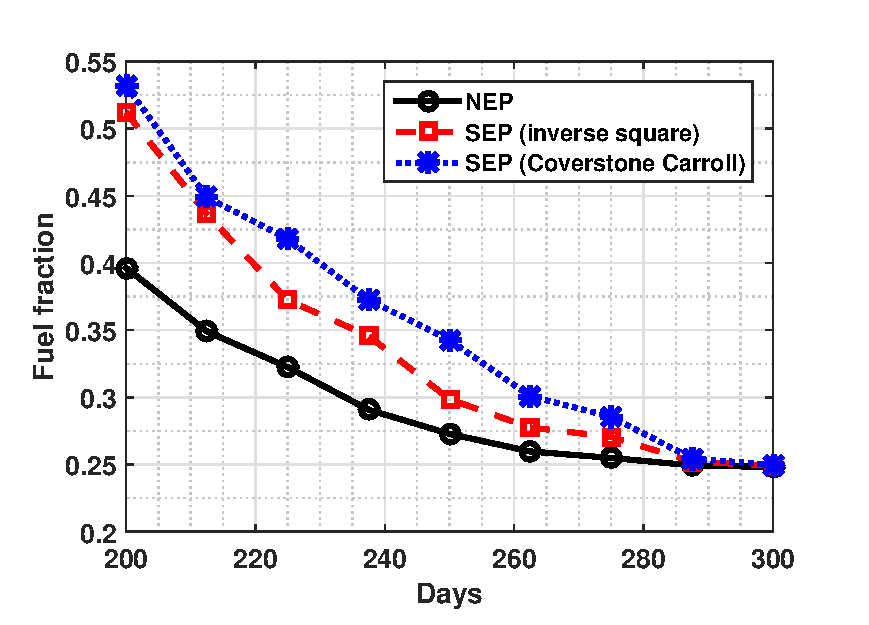
\includegraphics[width=1.00\linewidth]{FuelOptParam.eps}
	\caption{Fuel fraction with flight duration.}
	\label{sc_fueloptparam}
\end{figure}
Figure \ref{sc_fueloptparam} shows the trend in propellant required with increasing flight duration. It is seen that with increase in flight duration, all power models require lower propellant mass. It is also visible that this trend stagnates at higher flight durations and all the three power models tend to converge to the same fuel fraction value. The primary advantage of NEP is in outward transfers with low flight durations. This is due to the rapid loss of the maximum available thrust that SEP models face at higher distances from the sun. This situation reverses during inward travel where equal performing SEP and NEP thrusters at the starting point will ensure that the SEP thruster outperforms NEP once the trajectory moves closer to the sun.
\section{Two dimensional elliptic to ellipse transfers}
For demonstration, a transfer from a fictitious 0.4AU perihelion orbit with eccentricity 0.5 to a 1.524AU perihelion orbit with eccentricity 0.1 is performed with NEP. The initial acceleration level is $1mm/s^2$ with 2000s $I_{sp}$. The angle between the line of apsides is 225 degrees. Figure \ref{ellipse-to-ellipse} illustrates this transfer. The spacecraft starts at the aphelion.
\begin{figure}[H]
	\centering\includegraphics[width=1.00\linewidth]{Trajec_ellipseToCircle.eps}
	\caption{A typical ellipse to ellipse transfer.}
	\label{ellipse-to-ellipse}
\end{figure}
\subsection{Parametric studies - Impact of start location}
\subsubsection{Time-optimal ellipse-circle transfer}
Here, a transfer is considered from the 0.4AU perihelion, 0.5 eccentricity orbit to a 1.524AU circular orbit around the sun with NEP. The initial acceleration is $1mm/s^2$ with 2000s $I_{sp}$. the starting location is varied on the initial elliptic orbit. The fuel fraction and transfer angle geometry is seen to be a strong function of this starting true anomaly on the initial orbit. A swing of about $25\%$ is seen in the required fuel fraction in these transfers.\\
Figure \ref{ellipse-to-circ_fuel} shows the fuel fraction needed with varying initial true anomalies in the time-optimal framework. It is seen that the maximum propellant consumption occurs when the spacecraft starts in the vicinity of the perihelion. The minimum occurs at a true anomaly of approximately $120^\circ$. This plot reveals that from such an orbit, it may be preferable to coast initially until the optimum true anomaly is attained. This information is obtained without having to solve the numerically difficult fuel-optimal problem.
\begin{figure}[H]
	\centering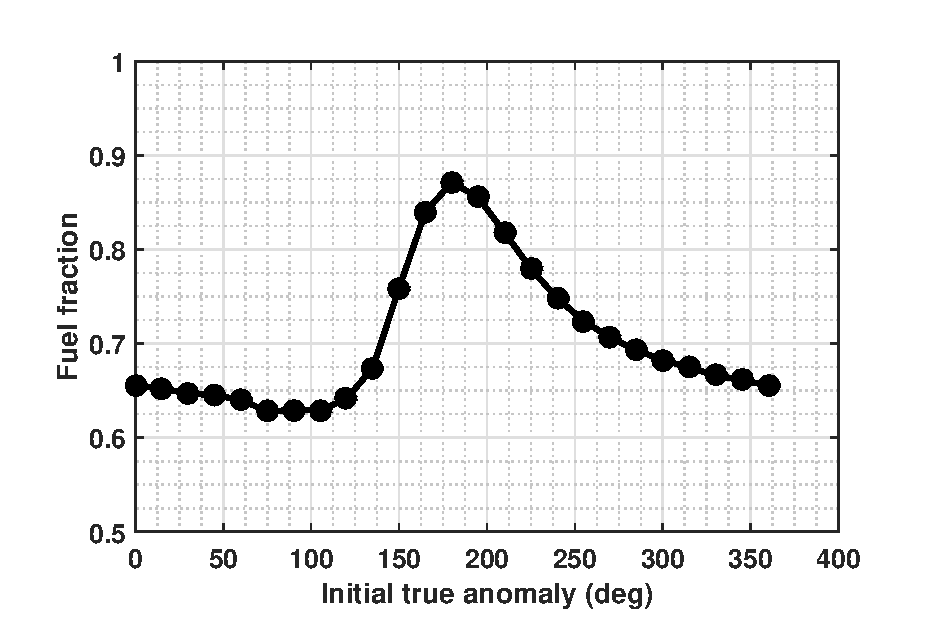
\includegraphics[width=0.90\linewidth]{FuelFrac_vs_trueAnomaly_final.eps}
	\caption{Fuel fraction variation with initial true anomaly in an ellipse to circle transfer.}
	\label{ellipse-to-circ_fuel}
\end{figure}
\begin{figure}[H]
	\centering\includegraphics[width=0.90\linewidth]{TransferAngle_vs_trueAnomaly_final.eps}
	\caption{Transfer geometry variation with initial true anomaly in an ellipse to circle transfer.}
	\label{ellipse-to-circ_trantime}
\end{figure}
\begin{figure}[H]
	\centering\includegraphics[width=0.90\linewidth]{TransAngle_vs_Fltdur.eps}
	\caption{Transfer angle vs flight duration variation in an ellipse to circle transfer.}
	\label{ellipse-to-circ_trangle_trantime}
\end{figure}
Figure \ref{ellipse-to-circ_trantime} reveals a tentative reason for the minimum fuel consumption at $120^\circ$ initial true anomaly. It is seen that the transfer angle needed for this case is a minimum. This observation must be made with caution as a similar result is not seen at transfers from the aphelion. Even though at $250^\circ$ true anomaly, the transfer angle reaches a maximum, the fuel consumption for transfers from this location is not high as the spacecraft is now in the vicinity of the perihelion where it moves rapidly and the transfer is completed faster than those from the aphelion. The peak fuel consumption depending on when the combination of initial radial distance from the sun and transfer geometry take on the most unfavorable values rather than the value of any individual parameter. Figure \ref{ellipse-to-circ_trangle_trantime} shows that the minimum transfer time solution also corresponds to the minimum transfer angle. The solution with the largest transfer time also requires the largest  transfer angle. There are two solutions to every flight duration because the transfer can occur from the vicinity of the aphelion and the perihelion of the initial orbit but the transfer angle change is  vastly different. This is because the spacecraft is traveling much faster in the vicinity of the perihelion leading to larger transfer angles for the same flight duration.
\subsubsection{Fuel-optimal ellipse-circle transfer}
Here, 225 day transfers from between the same orbit as in the previous case are considered.
\begin{figure}[H]
	\centering\includegraphics[width=0.90\linewidth]{MinFuel_from3D.eps}
	\caption{Fuel fraction variation with initial true anomaly in an ellipse to circle transfer.}
	\label{ellipse-to-circ_minfuel}
\end{figure}
\begin{figure}[H]
	\centering\includegraphics[width=0.90\linewidth]{MinFuelCoast_from3D.eps}
	\caption{Coast duration variation with initial true anomaly in an ellipse to circle transfer.}
	\label{ellipse-to-cir_coast}
\end{figure}
In figure \ref{ellipse-to-circ_minfuel}, it is visible that the maximum fuel expenditure occurs when the start location is the aphelion. Nonetheless, it is seen that in comparison to the time-optimal case, as the transfer time is larger, the peak is of a lower magnitude than in figure \ref{ellipse-to-circ_fuel}. Unlike the time-optimal case, for a wide range of starting true anomalies ($\pm 100^\circ$ from the perihelion), it is seen that the fuel fraction remains relatively insensitive to the starting location. This is because the coast is able to adjust for the disadvantageous starting location. 
Figure \ref{ellipse-to-cir_coast} shows the variation of the coast duration. For the $\pm 100^\circ$ range about the perihelion, the coast is greater than or equal to 120 days. When the starting true anomaly is in the vicinity of the aphelion, the total coast duration sharply drops to less than half the maximum value attained. This is the reason for the increase of over $25\%$ in propellant consumption compared to the minimum value.

\subsection{Trajectory with multiple intermediate coasts}
Figure \ref{Multcoasts} illustrates an ellipse-ellipse transfer from a 0.4AU perihelion orbit with eccentricity of 0.5 to a 1.524AU orbit with eccentricity of 0.1. The angle between the line of apsides is $225^\circ$. Figure \ref{Multcoasts_angle} shows the control profile. Two coast phases are clearly visible. 
\begin{figure}[H]
	\centering\includegraphics[width=0.90\linewidth]{Traj_multiplecoasts.eps}
	\caption{A typical trajectory with multiple intermediate coasts.}
	\label{Multcoasts}
\end{figure}
\begin{figure}[H]
	\centering\includegraphics[width=0.90\linewidth]{MultipleCoasts.eps}
	\caption{Control profile for the trajectory with multiple intermediate coasts.}
	\label{Multcoasts_angle}
\end{figure}
The first and last thrust phases have inward radial components. The second thrust phase is mostly tangential. The first thrust phase also has a small retrograde component that leads to the lowering of the perihelion. This is an artifact of fixing the transfer duration to 225 days. Increasing the flight duration will alleviate this perihelion lowering which is a symptom of energy wastage. The above trajectory is the reason for the specification that the numerical method should be able to perform the trajectory optimization without any information a priori about the control structure. Depending on the flight duration, there may be multiple thrust-coast-thrust switchings that cannot be determined beforehand. 
\section{Three dimensional transfers}
\subsection{Typical 3D transfer}
To demonstrate the capability of the code, a 350 day fuel-optimal NEP transfer is considered from a 1AU circular orbit with $0^\circ$ inclination to a 0.5AU circular orbit inclined at $90^\circ$ to the initial orbit. This type of trajectories could be useful for closely observing the solar poles without having to resort to inclination change techniques that rely on gravity assists from Jupiter.
\begin{figure}[H]
	\centering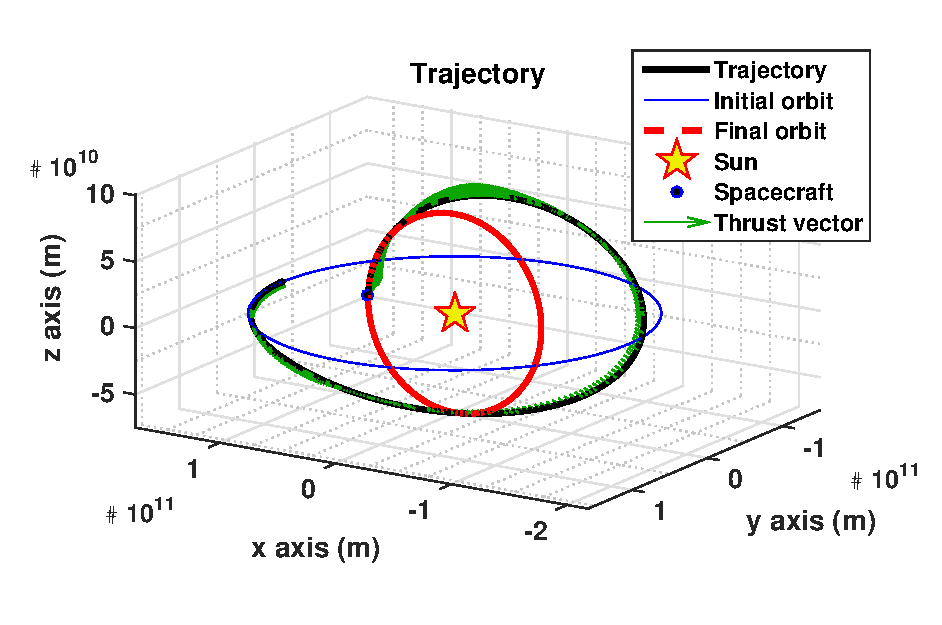
\includegraphics[width=0.90\linewidth]{3DTraj.eps}
	\caption{A typical 3D heliocentric trajectory.}
	\label{3d_Trajsample}
\end{figure}
As seen in figure \ref{3d_Trajsample}, the distance from the sun first increases and then it gets lowered to the final value.
\begin{figure}[H]
	\centering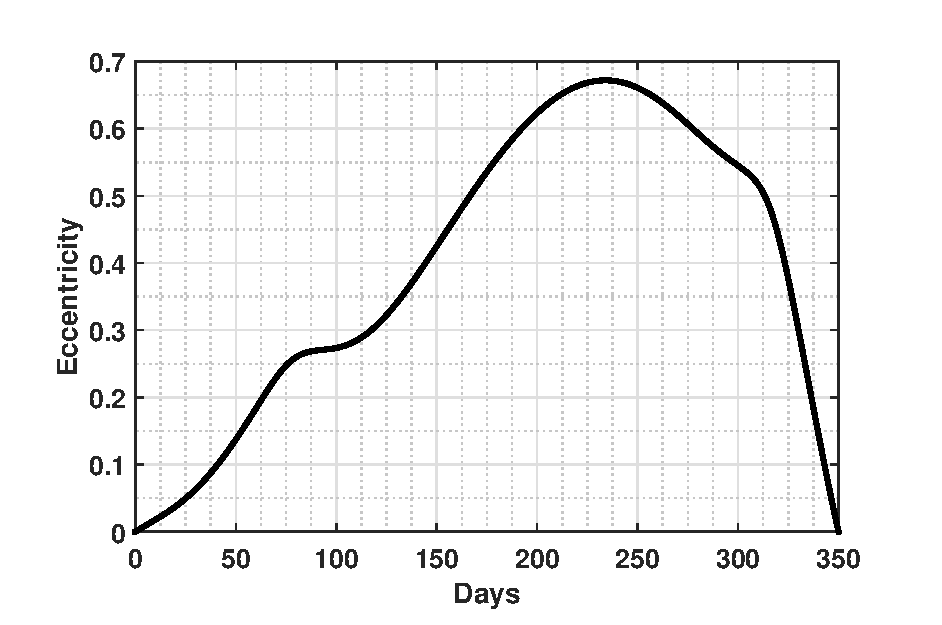
\includegraphics[width=0.90\linewidth]{3Deccen.eps}
	\caption{Instantaneous eccentricity profile.}
	\label{3d_sampeccenc}
\end{figure}
\begin{figure}[H]
	\centering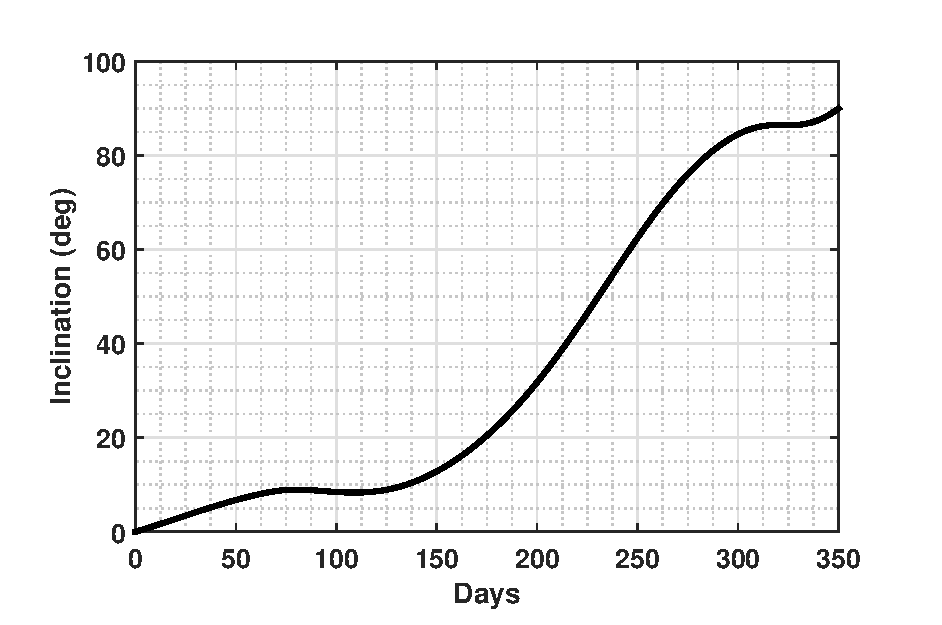
\includegraphics[width=0.90\linewidth]{3Dincl.eps}
	\caption{Instantaneous inclination profile.}
	\label{3d_sampincln}
\end{figure}
Figures \ref{3d_sampeccenc} and \ref{3d_sampincln} show the instantaneous eccentricity and inclination profiles for a typical transfer. When comparing with the trajectory plot, it is seen that the bulk of the inclination change occurs when the spacecraft is farthest from the sun. This is in accordance to conventional understanding as the $\Delta V$ requirements for inclination change is lowest when the spacecraft's velocity is a minimum. The final circularizing of the orbit occurs in the last phase of the trajectory when the spacecraft is very close to the final orbit. This is evident from the sharp drop in the eccentricity of the trajectory. The inclination only shows a minor change towards the target value in this time period. 
\subsection{Parametric studies on 3D transfers}
Three dimensional transfers include many variables, whose influence is difficult to qualitatively understand. For this purpose, the effect of inclination change on transfers between a 1AU to a 1.5AU circular orbit is studied in depth in order to obtain some understanding on the nature of such low thrust transfers. (Initial acceleration is taken to be $1mm/s^2$ with 2000s $I_{sp}$)
\subsubsection{With varying inclination, starting from nodal line}
\begin{figure}[h]
	\centering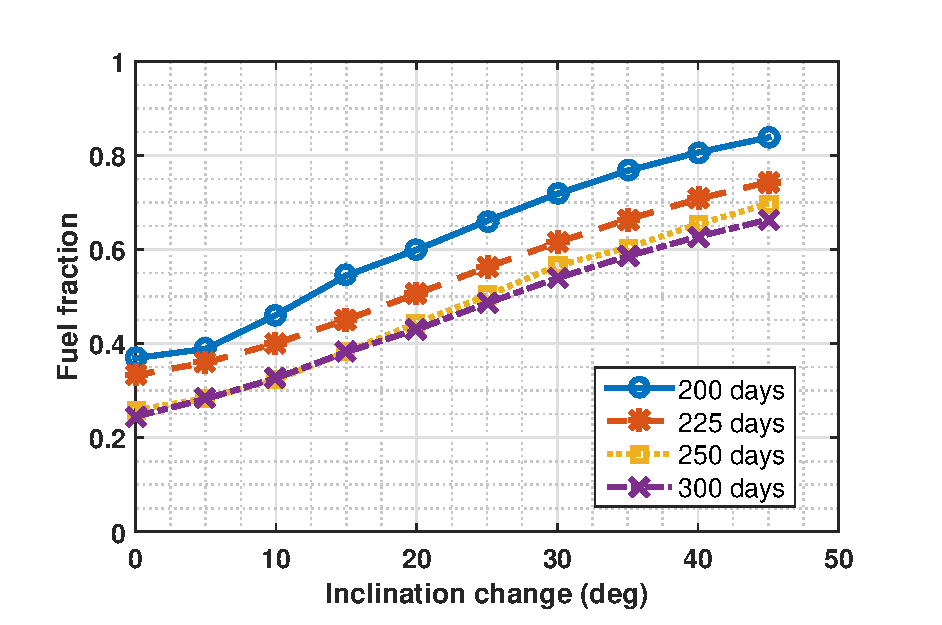
\includegraphics[width=0.80\linewidth]{3d_fuelfrac_vs_incln.eps}
	\caption{Fuel fraction with varying inclinations and flight durations.}
	\label{3d_varyincln}
\end{figure}
Here a spacecraft transfers between the aforementioned orbits with varying inclinations and flight durations in the fuel-optimal framework. The starting point is fixed on the line of intersection of the two orbital planes in the ascending side. The initial orbit is on the ecliptic plane. Figure \ref{3d_varyincln} shows the effect of both varying inclination change and the flight duration. It is clearly visible that higher inclinations lead to much greater propellant consumption. Increasing flight duration tends to reduce the propellant consumption but there is a lower bound as is evident from the figure. This means that increasing the flight duration will offer diminishing returns in terms of propellant requirements. These type of plots will enable designers to perform trade studies to analyze the best combination of propellant requirement and flight duration.
\subsubsection{Transfer between fixed orbits starting from different true anomalies}
\begin{figure}[h]
	\centering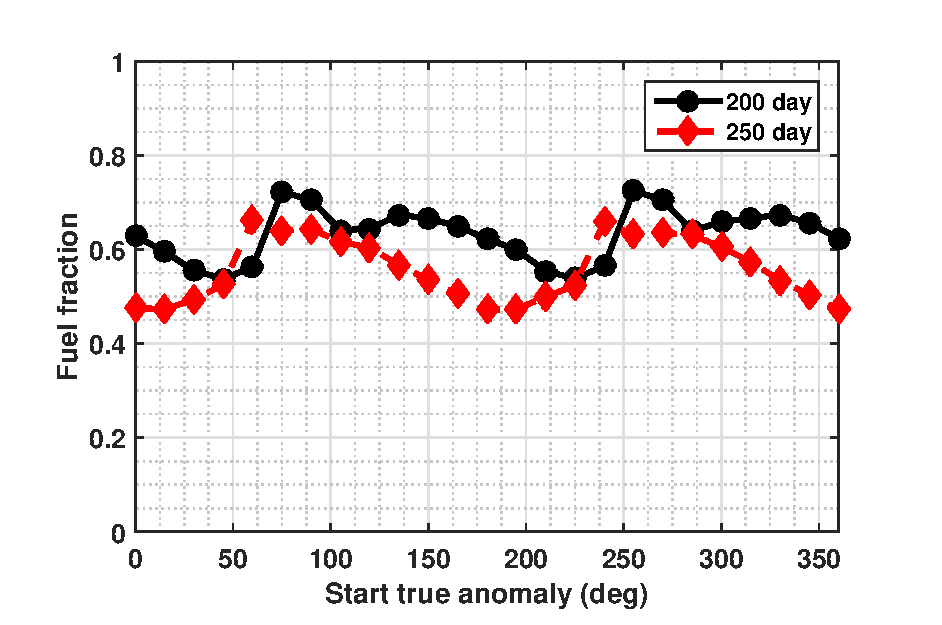
\includegraphics[width=0.80\linewidth]{3d_fuelfrac_vs_startpoint.eps}
	\caption{Fuel fraction with varying start locations.}
	\label{3d_varystart}
\end{figure}
Figure \ref{3d_varystart} presents results for the same spacecraft transferring from 1AU to 1.5AU with $22.5^\circ$ inclination change for a 200 and 250 day transfer. $0^\circ$ corresponds to a point on the line of intersection of the two circular orbital planes. There is roughly, a $20\%$ swing in fuel fraction needed depending on the starting location. In the minimum case, the majority of the inclination change is performed towards the final phase of the trajectory. This corresponds to an inclination change being performed in the vicinity of the line of intersection of the orbital planes. The maximum case corresponds to the inclination change being performed early. This corresponds to the conventional knowledge from impulsive transfers that a combined maneuver at the line of intersections of orbital planes farthest from the gravitating body leads to minimum $\Delta V$ requirements. The same seems to hold true in the case of low thrust maneuvers although it is impossible to comment about the exact nature of the maneuver and quantify it a priori to the trajectory optimization run.
Due to the circular nature of the initial and final orbits, the trends in figure \ref{3d_varystart} show a $180^\circ$ periodicity. The trajectories in the ascending and descending sides are identical all aspects except for the out of plane motion component which is inverted in sign. This type of periodicity is lost when the transfers happen between elliptic orbits or even if one of the orbits is elliptic. Even though there may be symmetry in the geometrical orientation, the kinetic energy of the spacecraft is vastly different between the periapsis and apoapsis sides of the elliptic orbit. This leads to only a $360^\circ$ periodicity in the more general case. 
\subsubsection{Issue with the solution}
It is also visible that for some starting true anomalies, the (example - at $60^\circ$ and at $240^\circ$) the 250 day transfer requires more propellant than the 200 day transfer. This is due to the non uniqueness of the solution. In the worst case, the solution that should have been found for the 250 day transfer at these points is actually a 200 day transfer followed by a coast once the final orbit is attained. In reality, these types of transfers are extremely difficult to obtain numerically. Thus for some cases, it is necessary to conduct extensive numerical experiments to determine the true nature of the solution. This occurs because the Pontryagin's minimum principle is only a necessary condition for optimality and does not guarantee uniqueness of the obtained optimal trajectories. This example serves to highlight the drawbacks of the solution procedure. Namely, fuel-optimality is not always guaranteed and the user must perform exhaustive analysis in case mission constraints are being violated.\\
The other alternative is to perform a wide range of numerical experiments and take the lower envelop of the resulting fuel fraction curves with their matching flight durations.
\subsubsection{Method to resolve the issue in the current framework}
In figure \ref{3d_varystart}, all the trajectories obtained have a thrust-coast-thrust control structure. There is only one coast duration in the middle phase of the trajectory. This is the result of rather wide boundss on the costate variables corresponding to the position. By tightening the bounds, a significantly better solution can be obtained.\\
Figure \ref{3d_varystart_tightcostates} presents the results of the repeated analysis with tighter bounds on the costates. The starting locations which previously led to higher propellant consumption for the 250 day case now lead to a net lower propellant consumption. The control structure for these trajectories is radically different different with a thrust-coast-thrust-coast-thrust structure. There are two intermediate coasts with one intermediate thrust phase. The inclination change is now performed at a location with better efficiency (i.e at the line of intersection of the orbital planes). 
\begin{figure}[H]
	\centering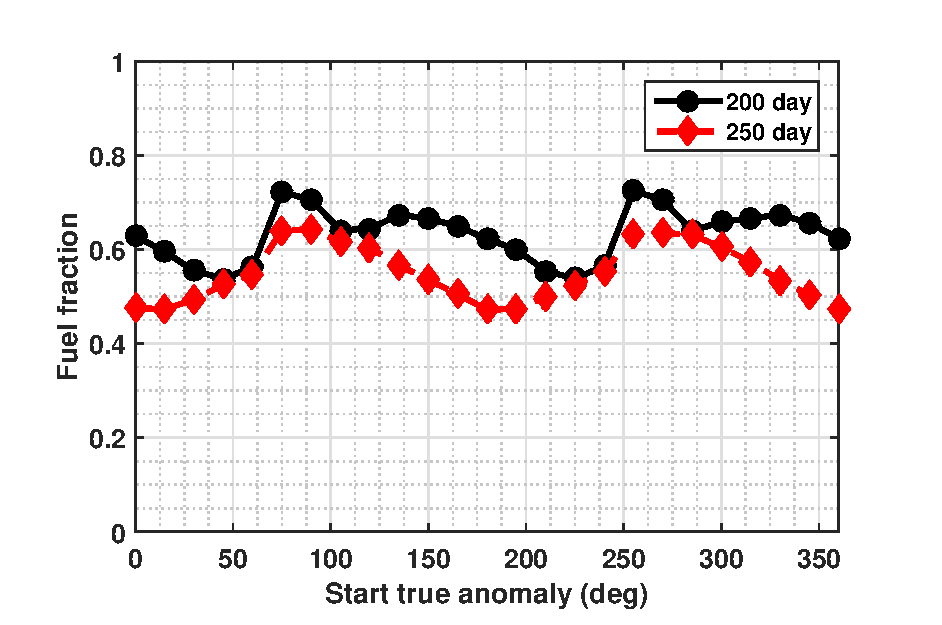
\includegraphics[width=0.80\linewidth]{3d_fuelfrac_vs_startpoint_tightcostates.eps}
	\caption{Fuel fraction with varying start locations (tighter costate bounds).}
	\label{3d_varystart_tightcostates}
\end{figure}
\begin{figure}[H]
	\centering\includegraphics[width=1.00\linewidth]{tightbounds_traj.eps}
	\caption{A 250 day trajectory starting at $60^\circ$ with tighter costate bounds.}
	\label{3d_traj_tightcostates}
\end{figure}
\begin{figure}[H]
	\centering\includegraphics[width=0.80\linewidth]{tightbounds_incln.eps}
	\caption{Inclination profile with tighter costate bounds.}
	\label{3d_traj_tightcostates_incl}
\end{figure}
The other starting true anomaly locations lead to the same trajectory with identical control structures and fuel consumption. This leads to the following strategy for the application of differential evolution to fuel-optimal transfers. If in the case of a larger flight duration, worse performing solutions are found, the bounds on the costate variables are to be progressively tightened until a better performing solution is found. In case no better solutions are found, it can be concluded (but not proven) that the best solution is the one with the lower flight duration followed by a terminal coast. It is seen from figure \ref{3d_traj_tightcostates} that the initial and final thrust phases operate mostly in plane maneuvers to change the semi-major axis. The intermediate thrust phase in the vicinity of the line of intersection of the orbital planes is seen to cause most of the inclination change. This observation is supported by figure \ref{3d_traj_tightcostates_incl}.\\
Here it is seen that about $21.6^\circ$ of inclination change is performed by the  intermediate burn. The initial and final burns lead to very small inclination changes. The coasts are visible as the two flat portions of the graph where the inclination stays constant. This is due to Keplerian dynamics which causes the angular momentum vector to be conserved under the absence of thrust forces. 
